\newgeometry{left=0.8in,right=0.8in,top=0in,bottom=0.7in}
\chapter*{Welcome Message}
%\addchap{Welcome Message}
%\addstarredchapter{Welcome Message}
%\chaptermark{Welcome Message}
%\addcontentsline{toc}{chapter}{Welcome Message} \mtcaddchapter

\vspace{-5em}
\textbf{\Large Dear Delegates}\vspace{1em}

The College of Engineering of Peking University is delighted to host the 2017 SPHERIC Beijing International Workshop (or \textbf{SPHERIC Beijing 2017}). This is an important event of 2017 in the field of Smoothed Particle Hydrodynamics (SPH) and related particle-based methods.

The SPH European Research Interest Community (SPHERIC) was founded in 2005 as a Special Interest Group of the ERCOFTAC community and aims at encouraging and facilitating the spread of the method throughout Europe and the wider international community. Since that time, the SPHERIC community continues both to grow and to play an important role in helping the development of SPH for academia, industry and government organizations. SPH is one of the most exciting new areas in the field of computational methods and is opening up the possibility of research into fields that were beyond any modelling capability. 

The SPHERIC Beijing 2017 organization committee received abstracts from China, France, Germany, UK, Italy, Spain, Switzerland, Ireland, USA, Japan and Australia, while 56 abstracts were selected to present in the SPHERIC Beijing 2017. This demonstrates just how active the field is, with works ranging from traditional hydrodynamics to solids, fluid-structure interaction, high performance computing and industrial applications. 

The SPHERIC Beijing 2017 has been supported by the National Natural Science Foundation of China (NSFC), the Chinese Society of Theoretical and Applied Mechanics (CSTAM), Beijing Innovation Centre for Engineering Science and Advanced Technology (BIC-ESAT), Institute of Ocean Research and State Key Laboratory for Turbulence and Complex Systems of Peking University, and Beijing Paratera Technology Co. Ltd.  

It is a great pleasure to welcome you all to Beijing, and share a successful and enjoyable meeting with you.


\begin{flushright}
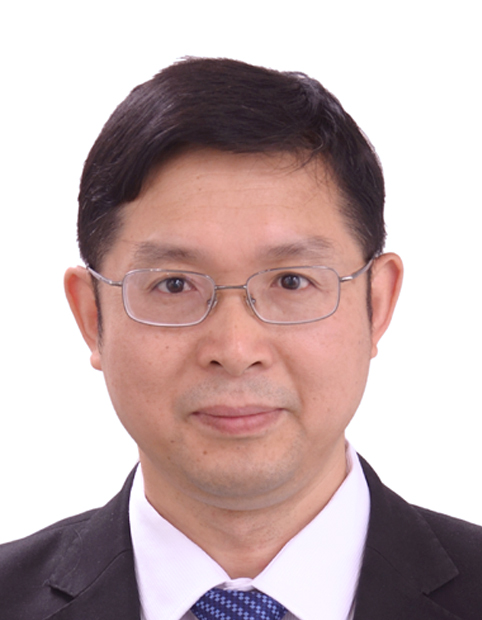
\includegraphics{mbliu.jpg}\\
\textbf{\MBLiu ~~~~~}\\
\vspace{1em}

Professor, Peking University\\
Chair, Local Organization Committee\\
SPHERIC Beijing 2017
\end{flushright}
\newgeometry{left=0.8in,right=0.8in,top=1in,bottom=0.7in}